\begin{figure}
    \centering
    \begin{subfigure}{.33\linewidth}
        \small
        \centering
        \begin{tikzpicture}[hypergraph,xscale=.7,yscale=.5,trim left=0cm,trim right=0cm]
            \node[vertex,label={east:$x_1$}] (x1) at (0, 0) {};
            \node[vertex,label={east:$x_2$}] (x2) at (-2, -2) {};
            \node[vertex,label={west:$x_3$}] (x3) at (2, -2) {};
            \node[vertex,label={east:$x_4$}] (x4) at (0, 0.75) {};
            \node[vertex,label={west:$x_5$}] (x5) at (-1, -1) {};
            \node[vertex,label={east:$x_6$}] (x6) at (1, -1) {};
            \node[vertex,label={west:$x_7$}] (x7) at (0, -2) {};
        
            \begin{scope}[on background layer]
                
                \newcommand*{\pathri}{($(x2) + (0,-0.4)$)
                    to[out=0,in=-135] ($(x5) + (-0.25,0.25)$)
                    to[out=45,in=180] ($(x1) + (0,-0.5)$)
                    to[out=0,in=135] ($(x6) + (0.25,0.25)$)
                    to[out=-45,in=180] ($(x3) + (0,-0.4)$)
                    to[out=0,in=0] ($(x4) + (0,0.5)$)
                    to[out=180,in=180] ($(x2) + (0,-0.4)$)
                }

                \newcommand*{\pathrii}{	($(x1) + (0.3,0.3)$)
                    to[out=135,in=45] ($(x5) + (-0.45,0.45)$)
                    to[out=-135,in=135] ($(x2) + (-0.3,-0.3)$)
                    to[out=-45,in=-135] ($(x5) + (0.45,-0.45)$)
                    to[out=45,in=-45] ($(x1) + (0.3,0.3)$)}
                
                \newcommand*{\pathriii}{($(x1) + (-0.3,0.3)$)
                    to[out=45,in=135] ($(x6) + (0.45,0.45)$)
                    to[out=-45,in=45] ($(x3) + (0.3,-0.3)$)
                    to[out=-135,in=-45] ($(x6) + (-0.45,-0.45)$)
                    to[out=135,in=-135] ($(x1) + (-0.3,0.3)$)}
                    
                \newcommand*{\pathriv}{	($(x2) + (0,0.4)$)
                    to[out=0,in=180] ($(x3) + (0,0.4)$)
                    to[out=0,in=90] ($(x3) + (0.5,0)$)
                    to[out=-90,in=0] ($(x3) + (0,-0.4)$)
                    to[out=180,in=0] ($(x2) + (0,-0.4)$)
                    to[out=180,in=-90] ($(x2) + (-0.5,0)$)
                    to[out=90,in=180] ($(x2) + (0,0.4)$)}
                
                \draw[hyperedge,looseness=.85, draw=BurntOrange,fill=BurntOrange,fill opacity=.1] \pathri;
                \draw[hyperedge,looseness=.85,draw=Red,fill=Red,fill opacity=.1] \pathrii;
                \draw[hyperedge,looseness=.85,draw=Fuchsia,fill=Fuchsia,fill opacity=.1] \pathriii;
                \draw[hyperedge,looseness=.85,draw=NavyBlue,fill=NavyBlue,fill opacity=.1] \pathriv;

                \node[text=BurntOrange] at (2,0.75) {$R_1$};
                \node[text=Red] at (-0.5,-1) {$R_2$};
                \node[text=Fuchsia] at (0.5,-1) {$R_3$};
                \node[text=Cyan] at (0.5,-2) {$R_4$};
                
            \end{scope}
        \end{tikzpicture}
        \caption{Query hypergraph}
        \label{fig:123-12-13-23-hg}
    \end{subfigure}
    \hfill
    \begin{subfigure}{.66\linewidth}
        \small
        \centering
        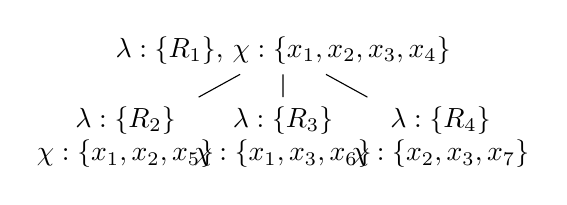
\begin{tikzpicture}[
			level distance=1.1cm,
			level 1/.style={sibling distance=2cm}
        ]
			\node { $\lambda: \{ R_1 \}$, $\chi : \{ x_1, x_2, x_3, x_4 \}$ }
				child { node[align=center] {$\lambda: \{ R_2 \}$ \\ $\chi: \{ x_1, x_2, x_5 \}$} edge from parent[-] }
                child { node[align=center] {$\lambda: \{ R_3 \}$ \\ $\chi: \{ x_1, x_3, x_6 \}$} edge from parent[-] }
                child { node[align=center] {$\lambda: \{ R_4 \}$ \\ $\chi: \{ x_2, x_3, x_7 \}$} edge from parent[-] } ;
		\end{tikzpicture}
        \caption{A join tree / hypertree decomposition}
        \label{fig:123-12-13-23-meta}
    \end{subfigure}
    \hfill\ 

    \hfill
    \begin{subfigure}{.32\linewidth}
        \centering
        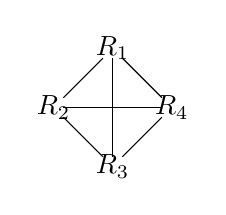
\begin{tikzpicture}[xscale=.75,yscale=.75]
            \node[label={center:$R_1$}] (R1) at (0,1) {};
            \node[label={center:$R_2$}] (R2) at (-1,0) {};
            \node[label={center:$R_3$}] (R3) at (0,-1) {};
            \node[label={center:$R_4$}] (R4) at (1,0) {};
            \draw (R1) -- (R2);
            \draw (R1) -- (R3);
            \draw (R1) -- (R4);
            \draw (R2) -- (R3);
            \draw (R2) -- (R4);
            \draw (R3) -- (R4);
        \end{tikzpicture}
        \caption{Query graph}
        \label{fig:123-12-13-23-qg}
    \end{subfigure}
    \hfill
    \begin{subfigure}{.32\linewidth}
        \centering
        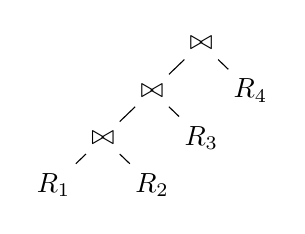
\begin{tikzpicture}[
			level distance=0.6cm,
			level 1/.style={sibling distance=1.25cm},
        ]
			\node { $\bowtie$ }
                child { node {$\bowtie$} edge from parent[-]
    				child { node {$\bowtie$} edge from parent[-]
                        child { node {$R_1$} edge from parent[-] }
                        child { node {$R_2$} edge from parent[-] }
                    }
                    child { node {$R_3$} edge from parent[-] }            
                } child { node {$R_4$} edge from parent[-] }
            ;
		\end{tikzpicture}
        \caption{A width-1 query plan}
        \label{fig:123-12-13-23-hierarchical-plan}
    \end{subfigure}
    \hfill
    \begin{subfigure}{.32\linewidth}
        \centering
        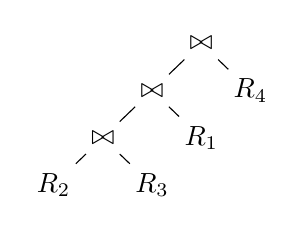
\begin{tikzpicture}[
			level distance=0.6cm,
			level 1/.style={sibling distance=1.25cm}
        ]
			\node { $\bowtie$ }
                child { node {$\bowtie$} edge from parent[-]
    				child { node {$\bowtie$} edge from parent[-]
                        child { node {$R_2$} edge from parent[-] }
                        child { node {$R_3$} edge from parent[-] }
                    }
                    child { node {$R_1$} edge from parent[-] }            
                } child { node {$R_4$} edge from parent[-] }
            ;
		\end{tikzpicture}
        \caption{A width-2 query plan}
        \label{fig:123-12-13-23-non-hierarchical-plan}
    \end{subfigure}
    \hfill\ 
    \caption{The hypergraph, a join tree, the query graph, and two query plans of the query $Q_{\ref{ex:123-12-13-23-intro}}$ in \cref{ex:123-12-13-23-intro}}
    \label{fig:123-12-13-23}
\end{figure}
